%!TEX root=seke.tex
% mainfile: ../seke.tex

\section{Background}

Stress testing projects should start with the development of a model for user workload that an application receives. This should take into consideration various performance aspects of the application and the infrastructure that a given workload will impact. A workload is a key component of such a model. The term workload represents the size of the demand that will be imposed on the application under test in an execution. The metric  used for measure a workload is dependent on the application domain, such as the length of the video in a transcoding application for multimedia files or the size of the input files in a file compression application \cite{Molyneaux2009}. 

Search-Based Testing is the process of automatically
generating test according to a test adequacy criterion,encoded as a fitness function, using search-based optimization algorithms, which are guided by a fitness function. The role of the fitness function is to capture a test objective that, when achieved, makes a contribution to the desired test adequacy criterion . Search–Based Testing uses metaheuristic algorithms to
automate the generation of test inputs. Metaheuristics are strategies that guide the search process to efficiently explore the search space in order to find optimal solutions  \cite{Afzal2009a}.

A common goal of stress search-based testing is to find workloads that produce execution times that exceed the timing constraints specified. If a temporal error is found, the test was successful. The application of evolutionary algorithms to  stress tests involves finding the best- and worst-case execution times (B/WCET) to determine whether timing constraints are fulfilled \cite{Afzal2009a}. 

IAdapter is a JMeter plugin designed to perform search-based stress tests. The plugin uses genetic algorithms, tabu search and simulated annealing in a collaborative mode (hybrid metaheuristic) \cite{Gois2016}. JMeter is a desktop application designed to test and measure the performance and functional behavior of applications. The JMeter tool can test an emulated class using Mock objects. A mock object is a dummy implementation for an interface or a class. A Mock Object is a substitute implementation for emulating other domain code. Basic mock object allows testing a unit faking the communication with collaborating objects. It should be simpler than the real code, not duplicate its implementation \cite{Brown2003}. 


% \vspace*{-.05in}
\section{Common performance application problems and performance antipatterns}
\vspace*{-.05in}

Performance is critical to the success of today’s software systems. Many software products fail to meet their performance objectives when they are initially constructed. There are several antipatterns that detailed features about  common performance problems. Antipatterns are conceptually similar to patterns in that they document recurring solutions to common design problems. They are known as
antipatterns because their use produces negative consequences.  Performance antipatterns document common performance mistakes made in software architectures or designs \cite{brown1998antipatterns}. Table \ref{antipatterns} present some of the most common performance antipatterns.

% Please add the following required packages to your document preamble:
% \usepackage{multirow}
% \usepackage[table,xcdraw]{xcolor}
% If you use beamer only pass "xcolor=table" option, i.e. \documentclass[xcolor=table]{beamer}
\begin{table}[h]
\centering
\caption{Performance antipatterns}
\label{antipatterns}
\begin{tabular}{|c|}
\hline
\rowcolor[HTML]{C0C0C0} \textbf{Antipattern}  \\ \hline
Blob or The God Class   \\ \cline{1-1}
Unbalanced-Processing \\ \cline{1-1}
Circuitous Treasure Hunt   \\ \cline{1-1}
Empty Semi Trucks   \\ \cline{1-1}
Tower of Babel   \\ \cline{1-1}
One-Lane Bridge   \\ \cline{1-1}
Excessive Dynamic Allocation   \\ \cline{1-1}
Traffic Jam   \\ \cline{1-1}
The Ramp    \\ \cline{1-1}
More is Less  \multirow{-10}{*}{} \\ \hline
\end{tabular}
\end{table}

Four antipatterns were chosen to this research  by the simplicity of implementation: Unbalanced-Processing, Circuitous Treasure Hunt, Tower of Babel and The Ramp.


A characteristic of Unbalanced Processing is the tendency to overload a particular resource. The overloaded resource will be executing a certain type of job very often, thus in practice, damaging other classes
of jobs that will experience very long waiting times.  Figure \ref{fig:unbalanced}  shows a sample of the Unbalanced Processing. In The Fig. \ref{fig:unbalanced}, four tasks are performed. The task D it is waiting for the task C conclusion that are submmited to a heavy processing situation. 


\begin{figure}[h]
\centering
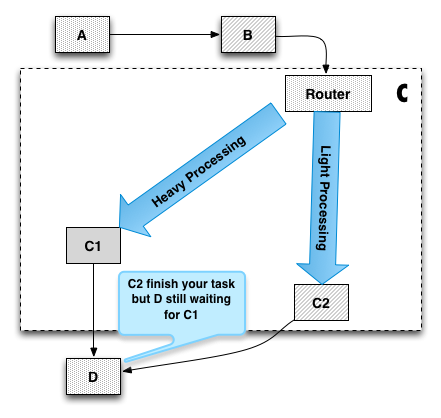
\includegraphics[width=0.4\textwidth]{./images/unbalanced.png}
\caption{Unbalanced Processing sample \cite{Wert2013a}. }
\label{fig:unbalanced}
\end{figure}

Circuitous Treasure Hunt antipattern occurs when software retrieves data from a first componet, uses those results in a second component, retrieves data from the second component, and so on, until the last results are obtained. Circuitous Treasure Hunt 
are typical performance antipatterns that causes unnecessarily high amount of frequent database requests \cite{Wert2014}. 

Tower of Babel antipattern most often occurs when information is translated into an exchange format, such as XML, where the sending process is then parsed and translated into an internal format by the receiving process. When the translation and parsing is excessive, the system spends most
of its time doing this \cite{Wert2014}.

\begin{figure}[h]
\begin{minipage}{.5\textwidth}
\centering
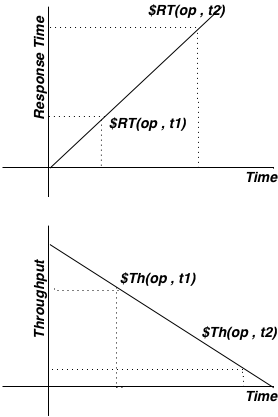
\includegraphics[width=0.5\textwidth]{./images/ramp.png}
\caption{The Ramp sample \cite{Vetoio2011}.}
\label{fig:ramp}
\end{minipage}
\end{figure}

Ramp is an antipattern where the processing time increases as the system is used. Fig. \ref{fig:ramp} shows a system  with the Ramp problem:  (i) the monitored response time of the operation opx at time t1, i.e. \$RT(opx, t1), is much lower than at time t2, i.e. \$RT(opx, t2), with t1 < t2; (ii) the monitored throughput of the operation opx at time t1, i.e. \$Th(opx, t1), is much larger than at time t2, i.e. \$Th(opx, t2), with t1 < t2 \cite{Wert2014}. 